\section{Mediciones}

Se realizaron mediciones en base a crear arreglos de diferentes largos, yendo de 100 en 100 elementos, donde los elementos en cada caso fueron generados por los valores pseudoaleatorios del lenguaje (el m\'odulo \texttt{random}). 

\begin{figure}[H]
    \centering % comparar el tiempo de ejecucion con (n log(n))
    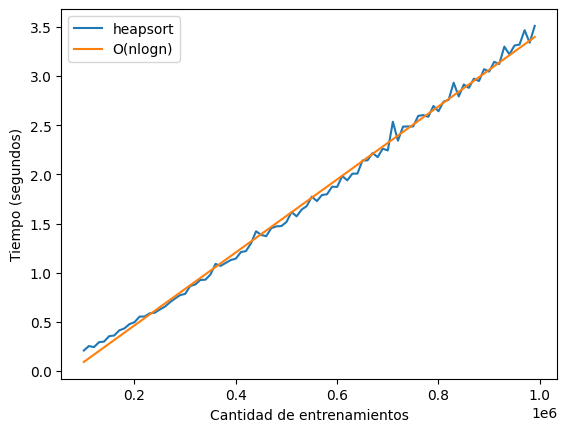
\includegraphics[width=1\textwidth]{img/tiempos.png}
\end{figure}

Como se puede apreciar, el algoritmo tiende a $\mathcal{O}\left(n \log n\right)$.
